\documentclass[10pt]{article}
\usepackage[T1]{fontenc}
\usepackage{lmodern}
\usepackage[margin=0.7in]{geometry}
\usepackage{amsmath}
\usepackage{microtype}
\usepackage{graphicx}
\usepackage{float}
\usepackage{booktabs}
\usepackage[font=small,labelfont=bf,skip=3pt]{caption}
\captionsetup[figure]{font=footnotesize}
\usepackage[dvipsnames]{xcolor}
\usepackage[colorlinks=true,linkcolor=MidnightBlue,citecolor=MidnightBlue,urlcolor=MidnightBlue]{hyperref}
\usepackage[capitalise]{cleveref}
\setlength{\parskip}{2pt}
\setlength{\parindent}{0pt}
\setlength{\intextsep}{6pt}
\makeatletter
\renewcommand\paragraph{\@startsection{paragraph}{4}{\z@}{1.0ex \@plus .3ex \@minus .2ex}{-1em}{\normalfont\normalsize\bfseries}}
\renewcommand\maketitle{\begin{center}{\large\bfseries\@title\par}\vspace{3pt}\@author\quad\textperiodcentered\quad\@date\end{center}}
\makeatother

\title{How AdamW and Muon Train a Small Language Model\\[1pt]
\normalfont Next steps (ii) and (iii) of the checkpoint}
\author{Juntang Wang}
\date{November 8, 2026}

\begin{document}
\maketitle
\vspace{-0.8em}

\paragraph{Summary.} (ii)~The update cosine follows the rule; so do stable rank and $\sigma_1/\sigma_{\mathrm{median}}$, but the spectral norm does not. (iii)~Weight decay does not explain Muon's speed; without orthogonalization Muon is worse; speed and spectra move together, so the cause is open; after a swap the loss moves before the stable rank.

%% =================================================================
%% Setup and reproduction
%% =================================================================
\section{Setup and reproduction}
\label{sec:setup}

TinyStories-10M on FAS RC Cannon, the checkpoint's settings (AdamW $2\cdot10^{-3}$, Muon 0.01, 10{,}000 steps, data orders 0 to 2); spectral metrics are means over the 36 block matrices. The rerun agrees (\cref{tab:repro}).

\begin{table}[H]
\centering
\small
\caption{Rerun (checkpoint in brackets); the last two rows at training loss 1.81.}
\label{tab:repro}
\begin{tabular}{l cc}
\toprule
 & AdamW & Muon \\
\midrule
final validation loss & 1.339 to 1.345 (1.344) & 1.308 to 1.310 (1.309) \\
step reaching AdamW's final validation loss & & 7250 to 7750 (7500) \\
stable rank of $W$ & $32.7 \pm 0.2$ ($33.0$) & $86.3 \pm 0.5$ ($86.2$) \\
active MLP units & $0.120 \pm 0.001$ ($0.120$) & $0.222 \pm 0.001$ ($0.222$) \\
\bottomrule
\end{tabular}
\end{table}

%% =================================================================
%% (ii) Direct result of Muon's updates, or emergent in training?
%% =================================================================
\section{(ii) Direct result of Muon's updates, or emergent in training?}
\label{sec:ii}

%% =================================================================
%% Rules without learning
%% =================================================================
\subsection{Rules without learning}
\label{sec:noise}

On synthetic gradients (noise, or a rank-4 signal plus noise), each rule updates one matrix for 10{,}000 steps (\cref{fig:noise}).

\textbf{Update cosine follows the rule:} on noise, 0.90 for AdamW and 0.66 to 0.76 for Muon, close to the real runs (0.89, 0.74).

\textbf{The spectra do not:} on noise the stable rank is unchanged; with the rank-4 signal both fall to about 4 (step 1000: AdamW 3.7, Muon 9.9).

\begin{figure}[H]
\centering
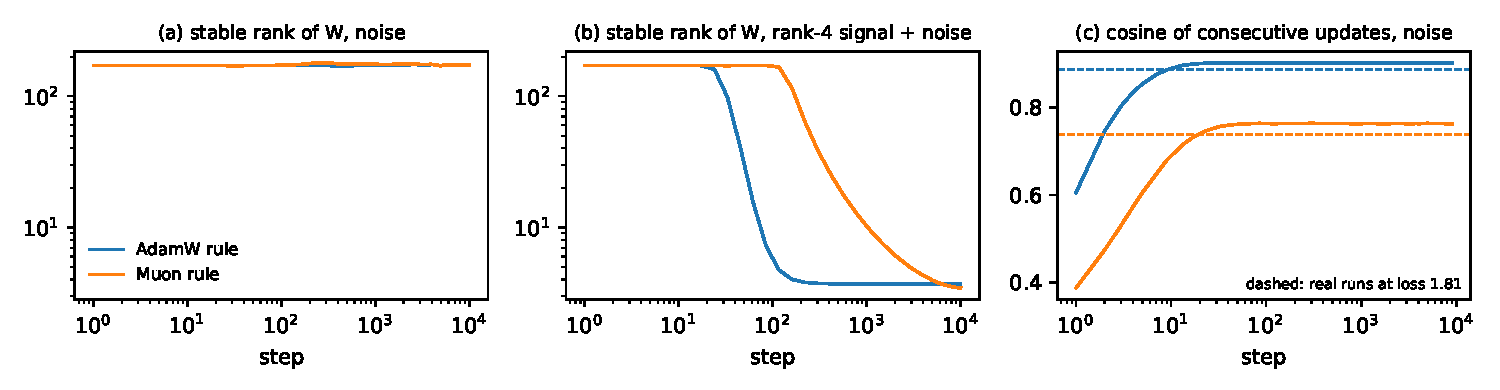
\includegraphics[width=\linewidth]{ts10m/rule_noise.pdf}
\caption{Each rule on synthetic gradients, MLP input matrix.}
\label{fig:noise}
\end{figure}

%% =================================================================
%% Ghosts on real gradients
%% =================================================================
\subsection{Ghosts on real gradients}
\label{sec:ghost}

\emph{Ghost}: a copy of the initial weights updated by the other rule on the run's own gradients, never fed back (\cref{tab:ghost,fig:ghost}).

\textbf{The ordering follows the rule:} on the same gradients Muon's rule gives the higher stable rank (87 against 40; 75 against 13).

\textbf{The spectral norm does not:} which rule is larger depends on the gradient stream (10.9 against 5.9 to 6.1; 7.5 against 7.7 to 7.8).

\begin{table}[H]
\centering
\small
\caption{The $2\times2$ design at step 10{,}000; range over data orders 0 to 2.}
\label{tab:ghost}
\begin{tabular}{l l ccc}
\toprule
rule & gradient stream & stable rank & $\sigma_1/\sigma_{\mathrm{median}}$ & update cosine \\
\midrule
AdamW & AdamW (run)  & 39.9 to 41.4 & 5.80 to 6.19 & 0.89 to 0.90 \\
AdamW & Muon (ghost) & 12.6 to 13.0 & 15.6 to 16.0 & 0.89 \\
\midrule
Muon  & Muon (run)   & 75.3 to 75.5 & 2.89 to 2.90 & 0.71 \\
Muon  & AdamW (ghost)& 87.0 to 87.2 & 2.77 to 2.80 & 0.70 \\
\bottomrule
\end{tabular}
\end{table}

\begin{figure}[H]
\centering
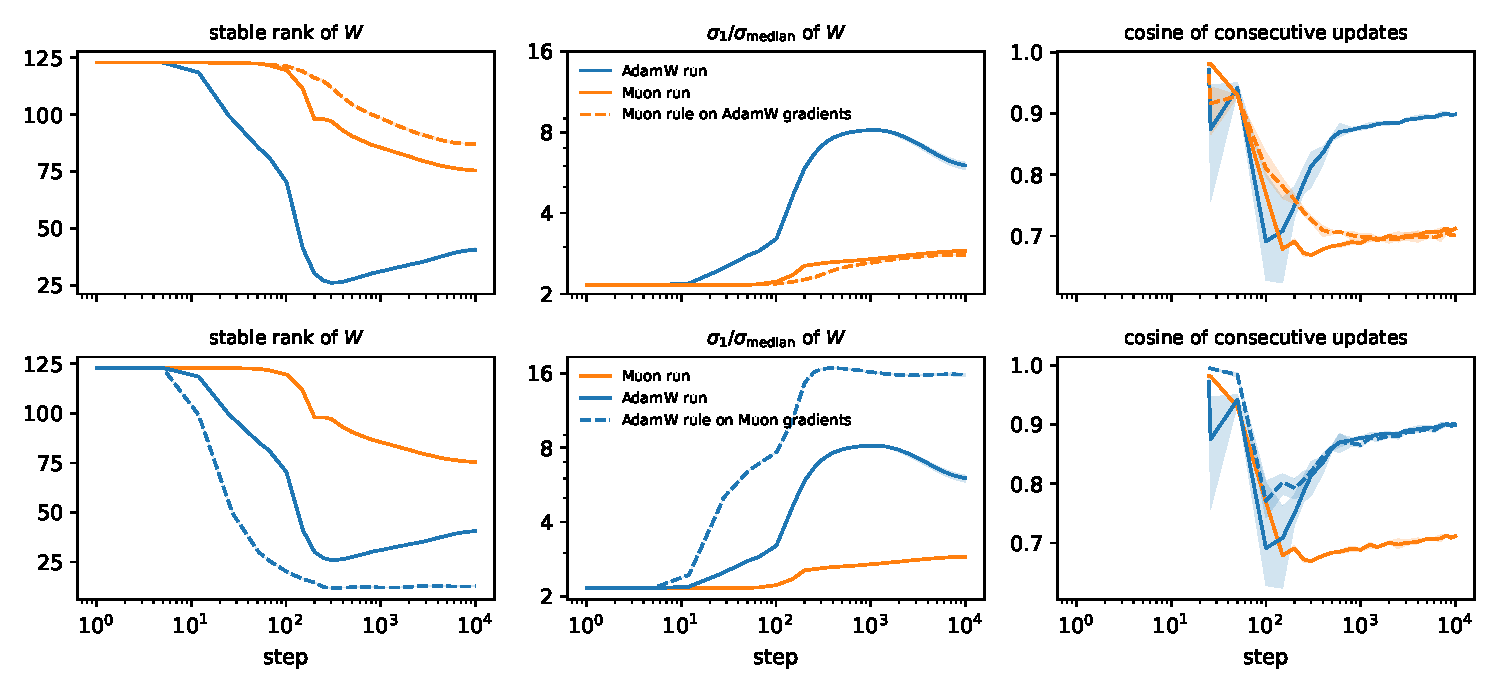
\includegraphics[width=\linewidth]{ts10m/ghost.pdf}
\caption{Ghosts (dashed) against runs; mean over data orders 0 to 2.}
\label{fig:ghost}
\end{figure}

%% =================================================================
%% (iii) Do the differences explain Muon's faster training and different path?
%% =================================================================
\section{(iii) Do the differences explain Muon's faster training and different path?}
\label{sec:iii}

%% =================================================================
%% What the speed needs
%% =================================================================
\subsection{What the speed needs}
\label{sec:ablate}

\textbf{Weight decay is not the reason (\cref{tab:ablate}):} Muon has none and is faster; adding or removing it changes final loss by 0.005 to 0.012.

\textbf{Without orthogonalization (momentum rescaled to an orthogonal update's norm) Muon is worse:} worse than AdamW at every learning rate; at 0.01 the two failing orders collapse to stable rank 3.6 and 5.5 (the order that trains: 34.8).

\begin{table}[H]
\centering
\small
\caption{Final validation loss at step 10{,}000.}
\label{tab:ablate}
\begin{tabular}{l ccc}
\toprule
run & \multicolumn{3}{c}{data order} \\
\cmidrule(lr){2-4}
 & 0 & 1 & 2 \\
\midrule
AdamW (baseline)                 & 1.339 & 1.341 & 1.345 \\
AdamW, weight decay 0            & 1.346 & 1.353 & 1.350 \\
\midrule
Muon (baseline)                  & 1.308 & 1.309 & 1.310 \\
Muon, weight decay 0.02          & 1.297 & 1.298 & 1.304 \\
\midrule
Muon, no orthogonalization, lr 0.01           & 3.729 & 2.943 & 1.389 \\
Muon, no orthogonalization, lr 0.003          & 1.454 &       &       \\
Muon, no orthogonalization, lr 0.03           & 4.078 &       &       \\
\bottomrule
\end{tabular}
\end{table}

%% =================================================================
%% Dose-response
%% =================================================================
\subsection{Dose-response}
\label{sec:dose}

Update singular values raised to $p$: $p=0$ is exact orthogonalization, $p=1$ none (\cref{tab:dose}; Muon, lr 0.01, order 0).

\textbf{Speed and spectra move together with $p$,} toward AdamW; the cause is open. $p=0.75$ on orders 0 and 1 is close to AdamW in stable rank and in the step reaching loss 1.81 (33.4 to 33.5 against 32.4 to 32.9; 1379 to 1394 against 1426 to 1469); order 2 stalls and ends at 1.659.

\begin{table}[H]
\centering
\small
\caption{Muon with singular values raised to $p$, data order 0; step and spectra at training loss 1.81.}
\label{tab:dose}
\begin{tabular}{l cccc}
\toprule
run & step at loss 1.81 & stable rank & $\sigma_1/\sigma_{\mathrm{median}}$ & final val.\ loss \\
\midrule
Muon (Newton-Schulz) & 846  & 86.6 & 2.68 & 1.308 \\
$p=0$ (exact SVD) & 827  & 88.2 & 2.64 & 1.306 \\
$p=0.25$    & 949  & 63.8 & 3.39 & 1.321 \\
$p=0.5$     & 1230 & 41.3 & 5.14 & 1.341 \\
$p=0.75$    & 1394 & 33.5 & 7.61 & 1.357 \\
\midrule
AdamW       & 1469 & 32.9 & 7.99 & 1.339 \\
\bottomrule
\end{tabular}
\end{table}

%% =================================================================
%% Swap timescale
%% =================================================================
\subsection{Swap timescale}
\label{sec:swap}

Swap rules at step $k$ (ORCD, order 0, compared only with the swap's own parents; \cref{fig:swap}).

\textbf{From step 1000 on, the loss moves before the stable rank:} AdamW to Muon, at $+100$ steps the loss gap is $-0.062$ (parents $-0.089$) while the stable rank has moved 9\%.

\textbf{Exception:} Muon to AdamW at step 400, the stable rank has moved 73\% by $+25$, together with the loss spike.

\begin{figure}[H]
\centering
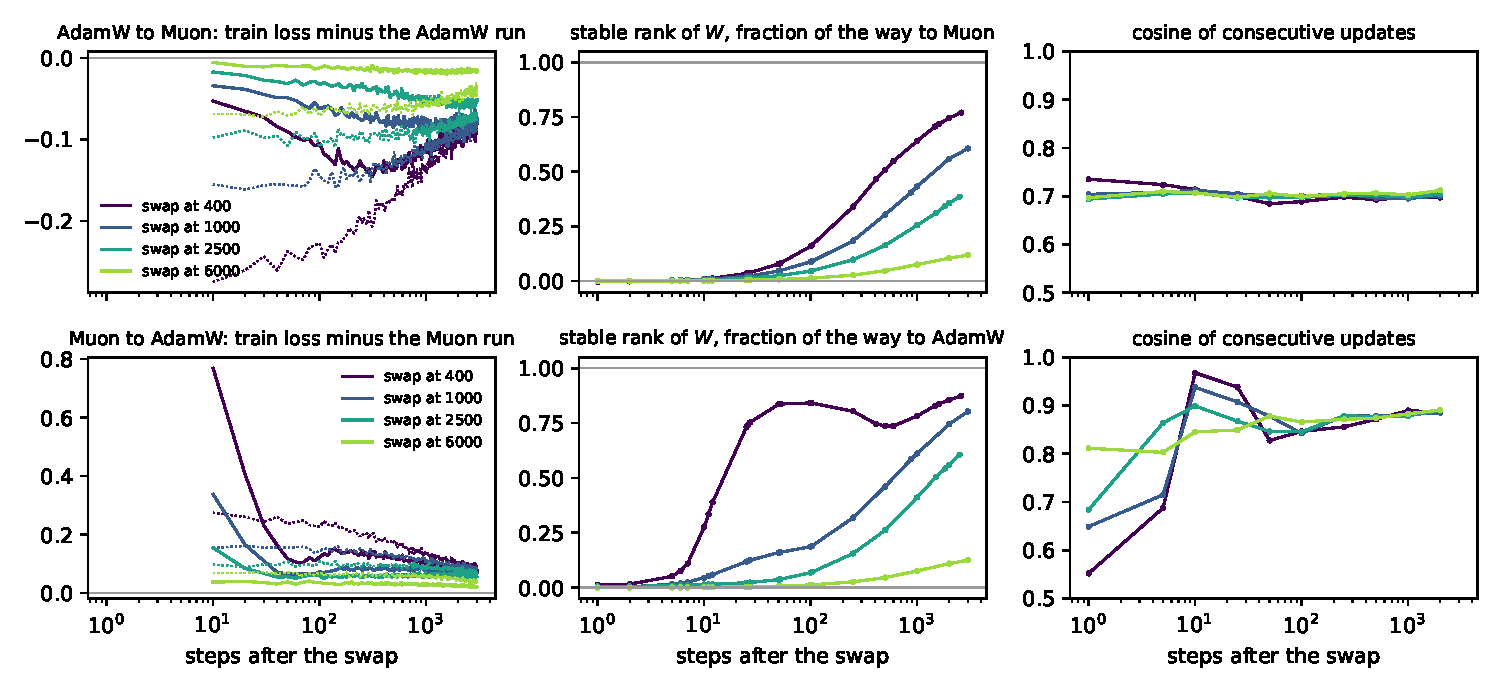
\includegraphics[width=\linewidth]{ts10m/swap_timescale.pdf}
\caption{Swaps at steps 400, 1000, 2500 and 6000. Dotted: the parents' loss gap.}
\label{fig:swap}
\end{figure}

\end{document}
